\chapter{Testgetriebene Entwicklung}
\label{sec:tdd}

\borderquote{TDD is also good for geeks who form emotional attachments to code. }{\cite{beck_test_2002}}Extreme Programming ist eine Agile Software-Entwicklungs Methodik, welche das Ziel hat, die Qualität der Software zu verbessern und flexibel auf Änderungen in den Anforderungen zu reagieren. Dazu implementiert sie einige Kernpraktiken. Eine Wesentliche, auf der viele der anderen Praktiken gründen, ist die "`Test-First"'-Praktik, die ab 2002 durch Kent Beck als Test-Driven-Development bekannt geworden ist \citep{beck_test_2002}.

Diese als Testgetrieben Entwicklung oder Test-Driven-Design bekannte Entwicklungstechnik basiert auf der Wiederholung von sehr kurzen Entwicklungszyklen, jeder nur wenige Minuten lang. Dabei ist es das Ziel, dass sich Test schreiben/Implementation und Refaktorisierungen, d.h. das konstante Verbessern des Systemdesigns und des Quellcodes, abwechseln. Mittlerweile werden die Begriffe Test-First Development und \glossar{TDD} oft synonym verwendet, allerdings gibt es manchmal Unterschiede in der Herangehensweise in Punkto Design der Software: TDD findet seine Anwendung, wenn nur eine vage Idee der Funktionalität einer Klasse besteht, während TFD kein Design oder Redesign der Klassen vorsieht, sondern dieses bereits im Vorfeld der Entwicklung stattfand \citep{stackoverflow_testing_2008}.

Im Folgenden wird die Entwicklungsmethode \glossar{TDD} näher beleuchtet und danach am Beispiel von Ruby\index{Ruby}/\glossar{rails} typische Testwerkzeuge aufzeigen.
\section{Motivation}
  Das Erstellen einer gut-abdeckenden \glossar{testsuite} ist für ein jedes größeres Softwareprojekt eine wichtige Voraussetzungen um interne Qualitäten, wie Wartbarkeit und Zuverlässigkeit zu aktivieren. \glossar{TDD} soll nicht dazu dienen, die Software zu validieren und die Umsetzung der funktionalen Anforderungen zu belegen. Das Hauptziel ist es nämlich, den Code in Einklang mit dem Test zu schreiben, so dass der Test den Code antreibt (Test drives the code), und letztendlich Design auf diese Art zum System hinzuzufügen. Die Auswirkung davon sei ein gut-testbarer Code, welcher in der Regel auch ein gut-wartbarer und verständlicher Code ist \citep{beck_test_2002}. \glossarpl{smell}, wie God-Methode und geringe Kohäsion, zu programmieren, wird alleine dadurch schon erschwert, da diese nur äußerst schwer zu testen sind.

  \paragraph{Psychologische Aspekte und Aspekte des Projektmanagements}

  Kent Beck beschreibt die Hauptmotivation für TDD, als das "`managing fear during programming"' Management von Angst. So hat Angst verschiedene Auswirkungen auf die Entwicklung. Sie mache zögerlich, führe zu weniger Kommunikation und damit Feedback und mache den Programmierer "`mürrisch"' \citep[S. xi]{beck_test_2002}.

  TDD fördert die Entwicklung in kleinen Schritten, und ermöglicht durch bestandene Tests kleine "`Belohnungen"' für den Programmierer. Dadurch ist es leichter einen gewissen Arbeitsrhythmus zu erhalten, was zu dem \textbf{Flow}\footnote{Schaffen-, Tätigkeitssrausch} führen kann\citep{roger_brown_test_2008} und damit eine effektivere Entwicklung ermöglicht.
  %Die Motivation für die Wahl von Test-getriebener Entwicklung als primäre Entwicklungsstrategie wird mit dem

  Falls TDD die Fehlerdichte signifikant verringern würde und nur Code entstünde, der getestet wurde, so hätte dies wohl auch soziale Auswirkungen auf die Software-Entwicklung\citep[S. x]{beck_test_2002}.
  \begin{enumerate}
   \item Die Qualitätssicherung könnte von einer reaktiven, auf eine proaktive Arbeit umstellen.
   \item Der Projektmanager kann den Ablauf der Entwicklung besser planen, da weniger überraschende Regressionsfehler im Laufe der Entwicklung auftreten
   \item Durch eine niedrige Fehlerdichte kann die Kontinuierliche Integration (Continuos Integration) möglich gemacht werden, und so der Kunde in den Entwicklungsprozess einbezogen werden
  \end{enumerate}



\section{Ablauf}
  Ziel ist es, vor der Implementation eines Codes, einen Unittest\index{Test!Unittest} (vgl. Abschnitt \ref{sec:testUnit}) zu implementieren. Davon ausgehend soll der geringstmögliche Code implementiert werden, damit der Test besteht. Als Letztes folgt die Refaktorisierung, bei TDD als Designphase genutzt. Danach beginnt der Kreislauf von neuem.

  \begin{figure}[htbp]
 \centering
 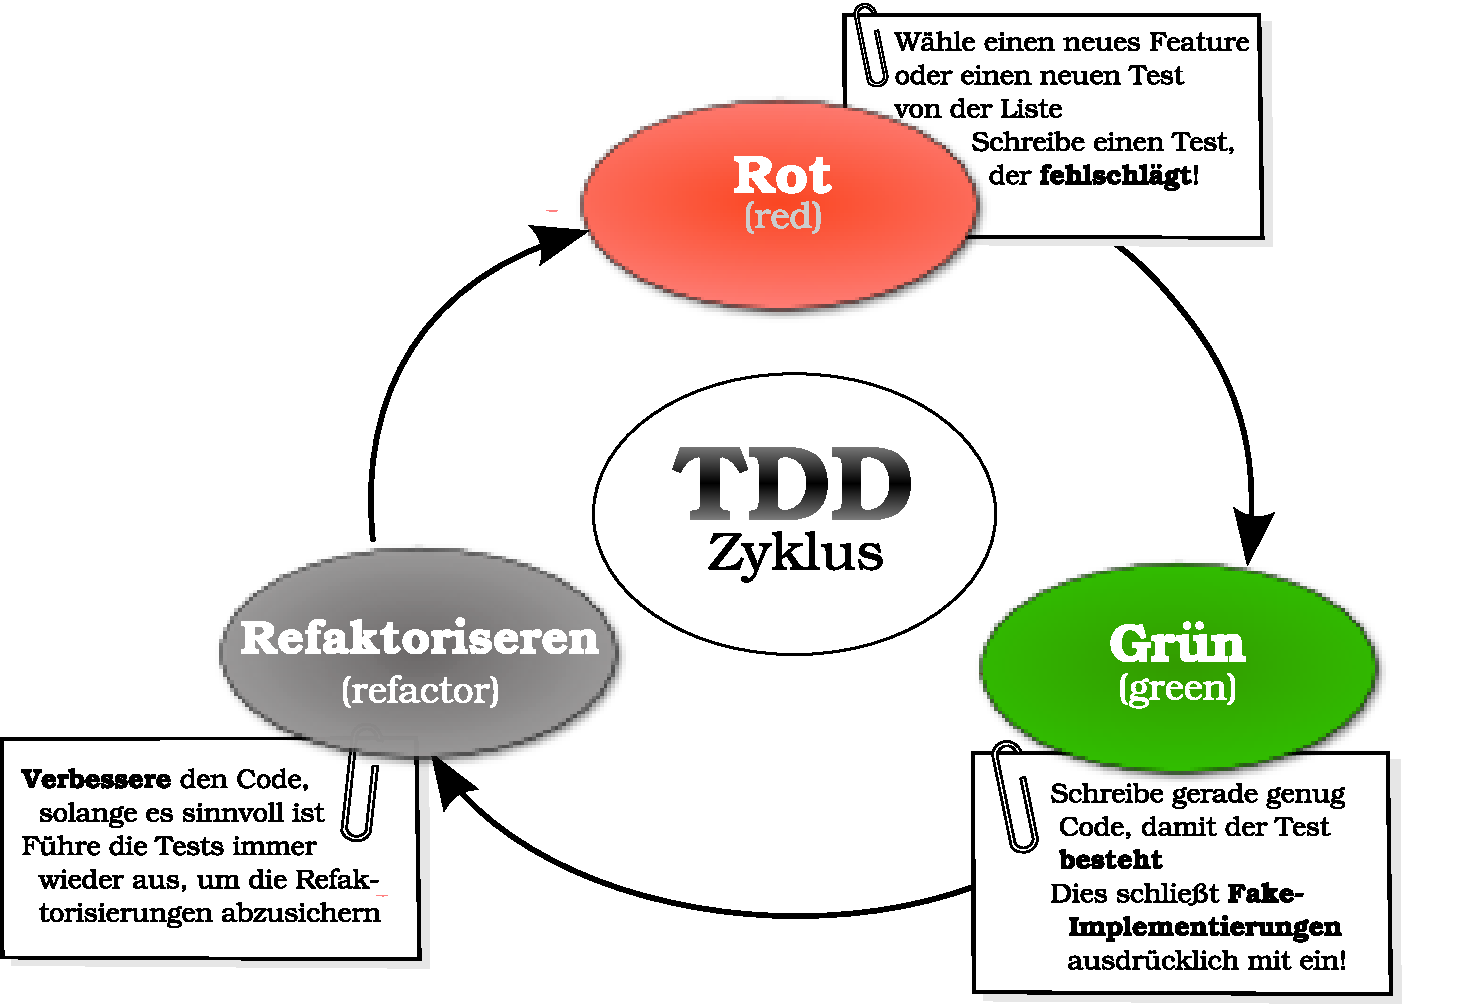
\includegraphics[width=0.85\textwidth]{./diagrams/red-green-refactor.pdf}
 % red-green-refactor.png: 884x602 pixel, 90dpi, 24.95x16.99 cm, bb=
 \caption{Red-Green-Refactor: Der TDD Entwicklungszyklus}
  \label{fig:redgreenrefactor}
\end{figure}
  Im Detail sind das also folgende Phasen, vgl. Abbildung \ref{fig:redgreenrefactor}:
  \begin{enumerate}
   \item Schreibe einen neuen \glossar{test}. Dies kann der erste eines neuen Features sein, oder aber ein weiterer Test, um das aktuelle Feature umzusetzen
   \item \textbf{Red}: Führe alle Tests aus, um sicherzugehen, dass der neue Test fehlschlägt. Andernfalls ist der Test überflüssig, da er keine neuen Informationen über das System gibt
   \item \textbf{Green}: Nachdem der Test fehlschlägt, implementiere nun den einfachsten Code, damit der Test besteht\\
   Dies kann ausdrücklich auch eine Fake-Implementierung sein, also z.B. die Rückgabe eines konstanten Wertes anstelle einer Berechnung. Wichtig ist, dass diese Phase so schnell wie möglich verlassen wird.
   \item \textbf{Refactor}: Nachdem der Test bestanden wird, folgt nun die \textbf{wichtigste Phase}, die Refaktorisierungsphase.\\
   Da wir bereits einen Test haben, der unser gewünschtes Systemverhalten widerspiegelt, können wir gefahrlos \glossar{refaktorisieren}, d.h. Design iterativ zum System hinzufügen und Duplikation zu eliminieren. Nun macht sich der Programmierer Gedanken, wie die vorhanden Klassen optimal refaktorisiert werden können, um \glossarpl{smell} zu eliminieren, und welches \glossar{patterns} ggf. angewendet werden kann.
  \end{enumerate}


  Ein genau spezifizierter Ablauf ist in Abbildung \ref{fig:tddflow} zu finden. Auch dort ist zu sehen, dass die Testerstellungs- und Refaktorisierungsphase strikt getrennt sind. Innerhalb ersterer solle nur möglichst schnell ein funktionierender Test erstellt und zum Bestehen gebracht werden. Die eigentliche Arbeit findet dann innerhalb der Refaktorisierungsphase statt, in der die wahrscheinlich suboptimale Implementierung verbessert wird, indem iterativ Design hinzugefügt wird.
  \begin{figure}[hp]
 \centering
 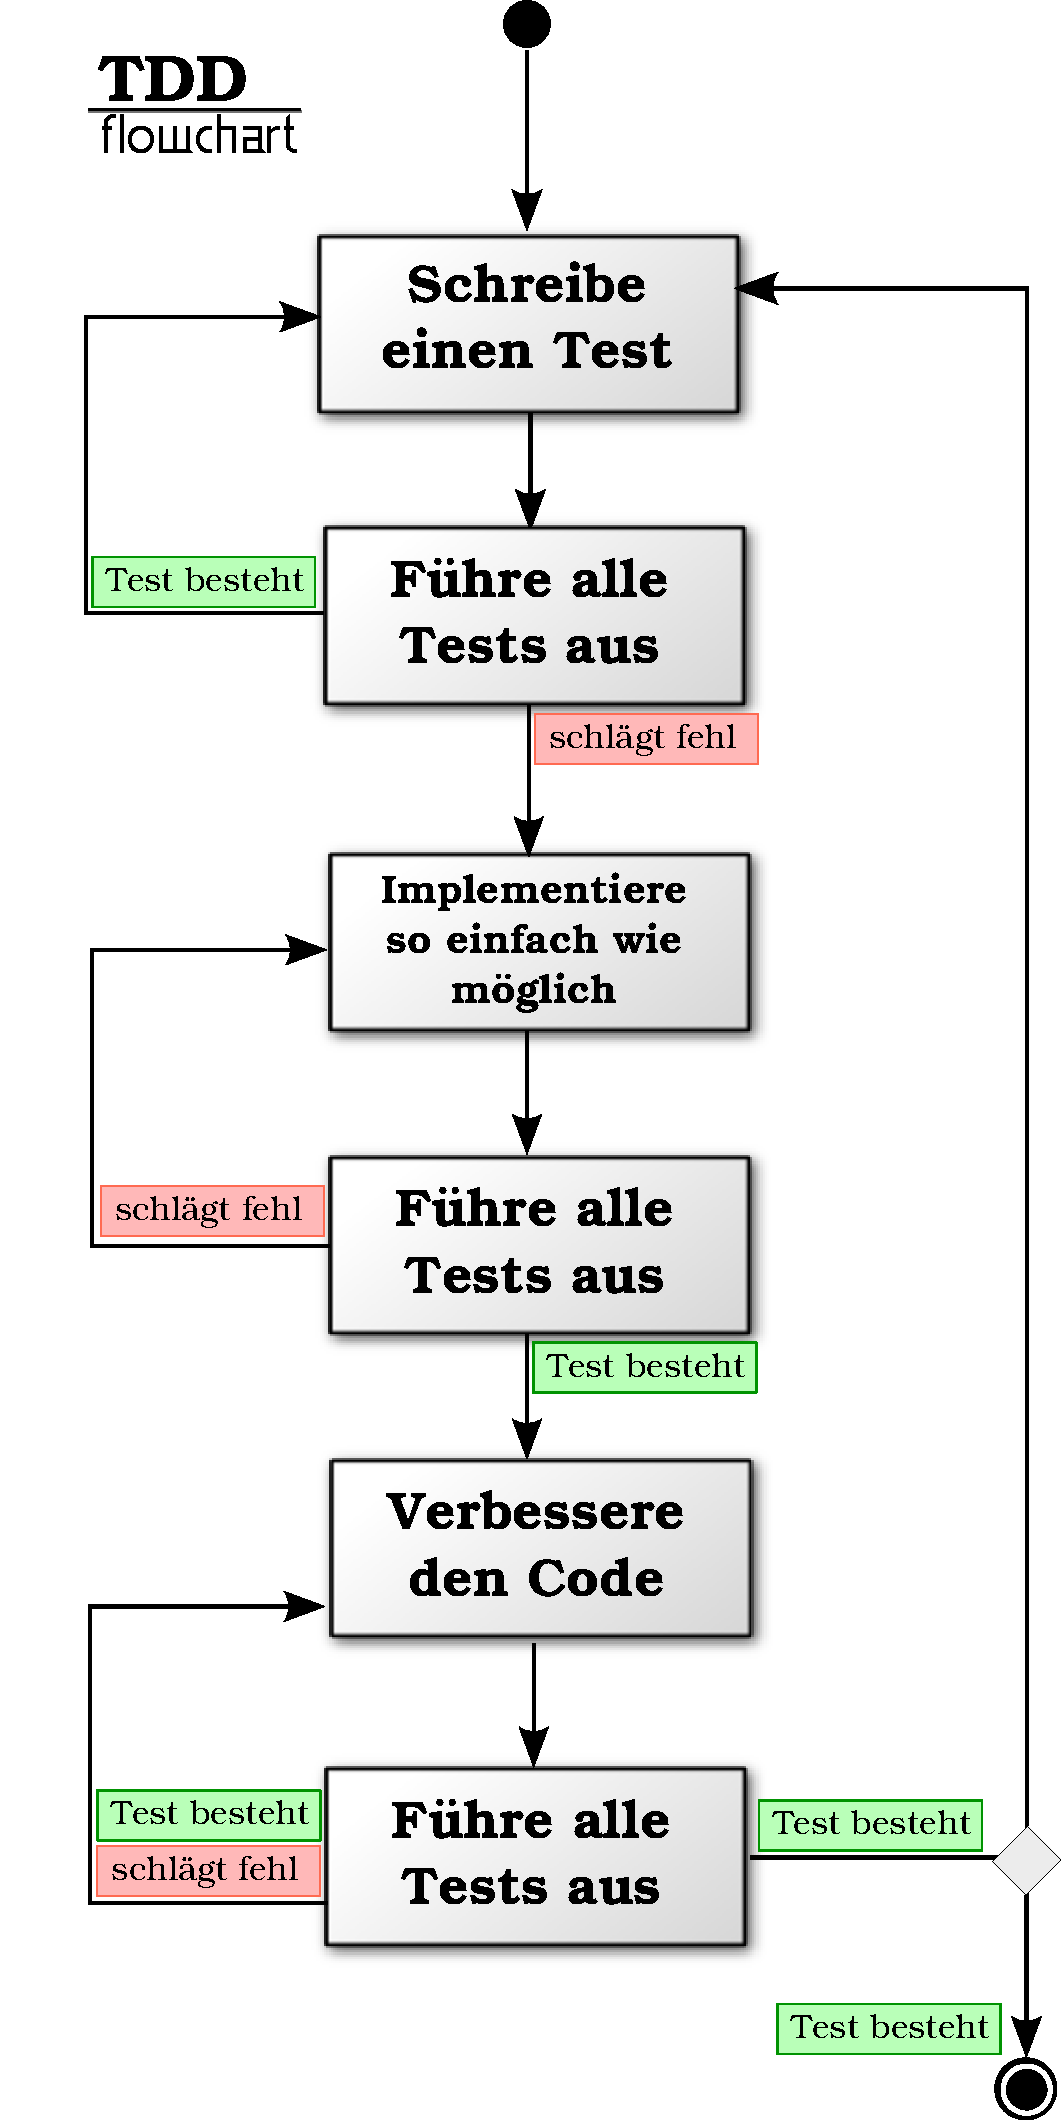
\includegraphics[width=0.6\textwidth]{./diagrams/tdd-flowchart.pdf}
 % tdd-flowchart.pdf: 510x1017 pixel, 72dpi, 17.99x35.88 cm, bb=0 0 510 1017
 \caption{Flussdiagram für TDD}
 \label{fig:tddflow}
\end{figure}


  Jeder Unittest\index{Test!Unittest} soll prinzipiell nur eine Eigenschaft testen, die Entwicklung erfolgt also in sehr kleinen Schritten. Dies hat direkte Auswirkungen auf die zu entwickelnden Objekte und Methoden, die dadurch ebenfalls übersichtlich werden sollen, und somit dem Objektbegriff, eine Klasse für eine Aufgabe, gerecht werden.

    \begin{figure}[hbtp]
 \centering
 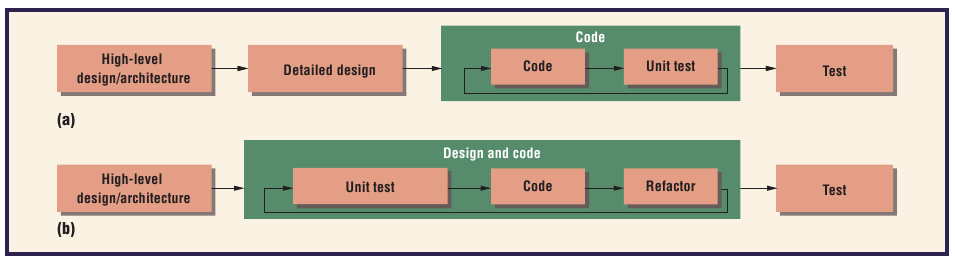
\includegraphics[width=\textwidth]{./diagrams/ablauf.png}
 % ablauf.png: 955x263 pixel, 96dpi, 25.26x6.96 cm, bb=0 0 716 197
 \caption{Entwicklungsablauf}
 \caption*{(a) Traditionelle Entwicklung,  b) Testgetriebene Entwicklung}
 \imgsource{Quelle: \citep{janzen_does_2008}}
 \label{fig:devflow}
\end{figure}

 TDD ist nur eine Entwicklungsmethodik. Der äußere Software-Entwicklungsprozess kann variieren und z.B. ein iterativer oder agiler Entwicklungsprozess sein. TDD lässt sich in einen solchen leicht einbetten, insofern der Prozess es erlaubt, das Design während der Entwicklung ändern zu lassen, und nicht schon vor den Iterationen festgelegt wird. Somit schreibt TDD nicht vor, wie eine Analyse oder ein vorhergegangener Grobentwurf, bzw. Architekturentscheidungen zustandegekommen sind.\borderquote{It's about the design, not the tests.}{Kent Beck}

 Innerhalb einer Iteration oder eines Durchlaufes des gewählten Vorgehensmodells, wird TDD an der Stelle des Design und der Entwicklung eingebettet, wie in Abbildung \ref{fig:devflow} dargestellt. Scheinbar wird so die (Fein-)-Design-Phase aus dem Ablauf entfernt. Stattdessen findet sie sich aber in Form der Refaktorisierung wieder.


  \section{Sonderfälle}
  \label{sec:tddspecialcircumstances}

  Der oben gezeigt Ablauf ist für den Normalfall, dem Entwickeln eines neuen Features, gedacht. Für einige gesonderte Problemstellungen im Programmieralltag existieren ebenso gewisse Abläufe.

  \paragraph{Fehlerbehebung} Falls trotz der Verwendung von \glossar{TDD} Fehler in der Software gefunden werden, so erfolgt:
  \begin{enumerate}
   \item Schreibe einen Test, der den Fehler auslöst bzw. nachbildet
   \item Behebe den Fehler im Programmcode
   \item Führe alle Tests aus
  \end{enumerate}
  Somit wird sichergestellt, das jeder bisher gefundene Fehler durch einen Test abgesichert wird, und jeder Programmfehler nur einmal auftritt.
  \paragraph{Spikes oder Spike Solution} In einigen Fällen ist es nicht ratsam, sofort mit einer Testgetriebenen Entwicklung zu beginnen. Gerade wenn Prototypisierung, d.h. schnelle, erforschende, explorative Entwicklung mit dem ausschließlichen Ziel schnell ein lauffähiges Ergebnis zu erhalten, gewünscht ist, dann kann auf Tests verzichtet werden. Eine solches, isoliert entwickeltes Experiment wird im \glossar{TDD}-Jargon \textbf{Spike} (zu deutsch: Spitze, Nadel) genannt. Die Idee dahinter ist es mehr über das Problem oder die zu erforschende Bibliothek zu lernen. Der produzierte Code sollte dann aber immer gelöscht werden und danach in originärer TDD-Manier neu entwickelt werden. Dies soll auch die gewählte Metapher einer Nadel aufzeigen: Schnell eine Nadel durch ein Brett bringen \citep{shore_art_2007}, als provisorische Lösung, die später durch eine besser designte ersetzt wird. Ausführliche Informationen über das Wann und Wie eines Einsatzes von Spikes finden sie in dem Buch "`The Art of Agile Development"' \citep{shore_art_2007}\footnote{Der Autor hat sogar das betreffende Kapitel online verfügbar gemacht \url{http://jamesshore.com/Agile-Book/spike_solutions.html}}.

  \paragraph{Testen von privaten Methoden/Attributen} Da die objektorienterte Modellierung das Konzept des Information Hiding und der Kapselung vorsieht, soll der interne Aufbau einer Klasse nach außen nicht sichtbar sein. Dies erreicht man mit den privaten Methoden und Attributen, die nur von Klasseneigenen Methoden benutzt werden dürfen. Da Tests aber von außen auf eine Klasse zugreifen, stellt dies scheinbar ein Problem dar. In einigen Sprachen löst man sich dieses Problem mittels Reflections, um über Umwege auf private Felder zuzugreifen. \\
  Dies spielt allerdings nur für das nachträgliche Testen von Legacy-Anwendungen eine Rolle. TDD in der Reinform betrieben sieht keine dedizierten Tests von privaten Methoden oder Attributen vor, da diese ausschließlich durch Refaktorisierung enstanden sein könnten \citep{caroli_agile_2008}. Die Tests der privaten Methoden erfolgt also nur implizit über das Testen der öffentlich-sichtbaren Methoden.


\section{Studien zu den Auswirkungen von TDD}

Viele Studien belegen, dass \glossar{TDD} positive Auswirkungen auf die Software-Entwicklung.

% Code Qualität

So zeigt eine Fallstudie, dass TDD zu größerer Produktqualität bei gleichzeitigt hoher Flexibilität führt, was ebenso in einer höheren Zufriedenheit bei den Programmiern führt \citep{hans_wasmus_evaluation_2007}.


Einer \randbem{Auswirkung auf die Code-Qualität}empirischen Studie zufolge, sei TDD schwierg zu erlernen und in einigen Metriken (Klassen pro Methode, Development Speed, Anteil der bestandenen Akzeptanztest\index{Test!Akzeptanztest}s) nicht signifikant besser als traditionelle Test-Last-Methoden. Allerdings hatten die beteiligten TDD-geführten Projekte eine signifikant bessere Testabdeckung und geringere Kopplung unter den Klassen. Test-First sei letztendlich eine mächtige aber kontraintuitive Technik \citep{madeyski_test-driven_2009}.


In dem Artikel des IEEE-Software-Journals stellen Janzen und Saiedian eine Studie vor, die akademische und industrielle Javaprojekte die testgetrieben durchgeführt wurden (Test-First), mit denen, bei denen hinterher getestet wurde (Test-Last), vergleicht. Demnach zeigen die Ergebnisse an, dass Programmierer, die einen Test-First Ansatz verfolgen, tendenziell Software in kleineren Einheiten die weniger komplex sind, schreiben, als solche die erst nach der Entwicklung testen \citep{janzen_does_2008}.


Einer \randbem{Auswirkungen auf die Struktur}anderen Studie nach, führt Testen im Allgemeinen dazu, dass weniger weniger Methoden verwendet werden und Klassen geringerer gekoppelt sind \cite{mueller_effect_2006}. Der Autor stellt auch eine potenzielle Metrik vor, um statistisch signifikant Projekte, die nach TDD betrieben wurden, von traditionellen Projekten zu unterscheiden: Assignment Controllability\footnote{Dies ist ein Maß, inwieweit der lokale Zustand einer Klasse/Methode von außen durch Parameter beeinflusst werden kann} \cite{mueller_effect_2006}. Allerdings rät der Autor zu weiteren Untersuchungen und setzt auch keinen Grenzwert an, ab welchem Grad der Controllability ein Projekt als TDD-Projekt bezeichnet werden kann.

% Verstaendnis

Einer \randbem{Verständnis von TDD in der Industrie}Umfrage unter 25 IT- und Entwicklungsleitern ergab, dass diese zwar die positiven Effekte unterstützen, aber nur 16\% TDD in der Praxis einsetzen, und nur 21\% Testvollständigkeit messen. Auch verstehen anscheinend etwa die Hälfte der Befragten den Begriff TDD falsch, nämlich als die reine Praxis Tests für alle denkbaren Problemfälle zu schreiben \citep{stelligent_inc_stelligent_2007}.

Das unter den Entwicklungsleitern der Fortune 500 Firmen, die von sich selbst behaupten, TDD zu betreiben, einige von Fehlannahmen ausgehen, wird in dem oben genannten Artikel genannt \citep{janzen_does_2008}. So setzen diese TDD mit automatisierten Tests gleich, oder behaupten sogar TDD sei das Schreiben ALLER Testfälle vor der Implementationsphase, anstelle der eigentlich gedachten kurzen Entwicklungs-Iterationen \citep{janzen_does_2008}.

% Auswirkungen auf Produktivit't und Bugs

Eine \randbem{Auswirkungen auf die Produktivität}Studie von Microsoft ergab, dass TDD-entwickelnde Teams eine 60\% -- 90\% geringere Fehlerdichte, aber eine 15\% -- 35\% längere Entwicklungszeit hätten, als nicht-TDD Entwickelnde \citep{nagappan_realizing_2008}.



\section{Prinzip des Emergent Design -- Inkrementelles Sofwaredesign}
\label{sec:tddEmergent}




%Dies stehe im Gegensatz zu einem klSoftware-Design, das im Vorfeld bedacht wurde
%discovering and harvesting patterns in existing Code
%GoF Patterns
%idiomatische Patterns: Patterns, die nur für genau eine Applikation oder innerhalb eines Unternehmens optimal sind. z.B. Security
%technical patterns
%domain patterns -> common business patterns
%emergent -> discover this
%traditional design -> too early, Business Process can change way faster, speculation without facts
%Frameworks sollten nicht designt werden, sondern sich aus Code ergeben
%im Gegensatz zu einer Ingenieurswissenschaftlichen Tätigkeit, das ... -> Iterativ
% ward cummingham
%http://www.developerdotstar.com/mag/articles/reeves_design.html
%http://confreaks.net/videos/282-lsrc2010-real-software-engineering
%http://www.ibm.com/developerworks/java/library/j-eaed5/index.html
%because you think about every little component that goes into the system
%cheap to build, expensive to design
%BDUF (Big Design Upfront)
%http://www.thoughtworks.com/emergent-design

Ein Konzept, das TDD effektiv macht, ist das sich Herausbildende Design (Emergent Design). Gegenüber traditionellen Entwicklungsansätzen erfolgt der Entwurf (Design) hierbei nicht als eigenständige Phase im Prozess, sondern ist streng in die Implementation integriert. Immer wenn ein Zyklus beim Refaktorisieren angelangt ist, findet nämlich effektiv Design statt. Eine Entwicklung nach TDD sucht den minimalsten Code, der die Anforderungen (Tests) erfüllt. Analog dazu, will ein Emergentes Design die kleinste Menge an benötigten Design suchen, die die Anwendung benötigt. Durch die vielen Iterationen und die darausfolgenden zahlreichen Refaktorisierungen tritt nach und nach das Design hervor, welches optimal für das System ist.


Einige \randbem{Gründe für eine Minimierung des Designs}Software-Architekten (\cite{neal_ford_emergent_2010,jack_reeves_three_1992,glenn_vanderburg_real_2010}) stellen fest, dass praktische Software\hyp{}Entwicklung kein Produktionsprozess ist, der sich nach herkömmlichen Methoden planen lässt. Dort sind Ingenieure für die Planung und das Design verantwortlich, welches in der Regel ausschließlich im Vorfeld der Implementierung stattfindet. Das klassische Software-Engineering empfindet diesen Prozess nach, und erstellt ein Design im Vorfeld der Entwicklung. Diese Autoren äußern nun, dass dies für die meisten Softwareprojekte nicht ideal sei, da sich die Businessanforderungen fast immer im Laufe einer Entwicklung ändern. Traditionelles Softwaredesign abstrahiere zu früh und spekuliere ohne die letztendlichen Fakten zu kennen. Die ingenieurswissenschaftliche Diszplinen hätten außerdem die Beschränkung, dass ein Build-Prozess äußerst teuer ist (man denke den Bau einer Brücke oder die Entwicklung von Flugzeugen), wohingegen Softwareentwicklung diese Beschränkung nicht besitzt, da ein Build meist (fast) nichts koste. Dadurch kann die Software-Entwicklung ein iteratives Vorgehen nutzen \cite{neal_ford_emergent_2010,glenn_vanderburg_real_2010,jack_reeves_three_1992}. Statt eines großen Designs am Anfang\footnote{(BDUF -- Big Design Upfront)} soll das Design durch Entdeckung und Extrahieren aus dem Sourcecode gewonnen werden.


Beim inkrementellen \randbem{Wie findet Abstraktion statt?}Design wird jedes Design-Artefakt, ob nun Methode, Klasse, Namespace oder sogar Architektur, nur deshalb erstellt, um ein bestimmtes, aktuelles Problem zu lösen. Dieses Design tendiert dazu, sich in Schüben zu entwickeln: Meist ändert man nur kleine Dinge, bis man durch eine Idee einen Durchbruch (Breakthrough) erzielt, und eine größe Abstraktion durchführt \cite{shore_art_2007,evans_domain_driven_2003}. Dies kann in allen drei Abstraktionsleveln, Methode, Klasse oder Architektur stattfinden.\\
Falls man \textbf{Paar-Programmierung} anwende, so ist es die Aufgabe des passiven Teilnehmers über das aktuelle Design zu reflektieren und Refaktoriserungen zu überdenken. Auf diese Weise können Durchbrüche auf Methoden-Level mehrmals pro Stunde stattfinden.\\
Während der Entwicklung, sollte der passive Teilnehmer der Paarprogrammierung ebenfalls darüber nachdenken, ob Ähnlichkeiten Ähnlichkeiten anderer Klassen zu der aktuell Entwickelten existieren. Falls er Redundanzien sieht, so solle er diese in einem passenden Refaktorisierungszyklus zur Sprache bringen. Beide Teilnehmer diskutieren dann mögliche Abstraktionen. Durchbrüche dieser Art können mehrmals pro Tag stattfinden (abhängig vom bereits vorhanden Design).\\
Ähnliches gilt dann im Architekturlevel, allerdings finden hier Durchbrüche nur alle paar Monate statt, und werden im gesamten Entwickler-Team diskutiert. Als Grundregel sollte man aber beim Einführen neuer Architekturelemente so konversativ wie möglich sein \citep{shore_art_2007}.

Ein Emergent Design kann auch ohne TDD in iterativen Entwicklungsprozessen verwendet werden. Allerdings ist die Umsetzung ohne das Vorhandensein einer guten Test-Suite ein risikoreiches Unterfangen. TDD sieht bereits eine Refaktoriserungsphase vor, und, zusammen mit einer Paarprogrammierung, bietet es damit perfekte Vorraussetzungen für ein inkrementelles Design.

\section{Varianten}
\subsection{ATDD -- Acceptance TDD}
\label{sec:attd}

Oftmals ist eine Dokumentation und automatisierte Prüfung der Anforderungen durch Akzeptanztest\index{Test!Akzeptanztest}s gewünscht. Hier findet die Akzeptanztest-getriebene Entwicklung als Modifikation von \glossar{TDD} ihre Anwendung. Statt der Unittest\index{Test!Unittest}s, stehen hier die Akzeptanztests im Vordergrund (vgl. \ref{sec:acceptance} zum Thema Akzeptanztests).

Die Entwicklung von Unittest\index{Test!Unittest}s lässt sich aber einbetten, wodurch man nun zwei Testebenen erhält \citep[S. 285]{chelimsky_rspec_2010}:

\begin{enumerate}
 \item Schreibe einen Akzeptanztest\index{Test!Akzeptanztest}/Systemtest für ein Szenario des Feature
 \item Prüfe, ob der Akzeptanztest\index{Test!Akzeptanztest} fehlschlägt
 \item Implementiere das Feature. Da die Features teilweise komplex sind, verfahre nun nach dem TDD-Schema, um benötigte Klassen zu entwickeln, die notwendig sind, um das Feature zu realisieren:
  \begin{enumerate}
   \item Schreibe einen Unittest\index{Test!Unittest}
   \item Prüfe, ob der Test fehlschlägt, andernfalls zurück zu 1.
   \item Implementiere mit so wenig wie Code möglich, so dass der Test besteht
   \item Refaktorisiere
  \end{enumerate}
 \item Nachdem der Akzeptanztest\index{Test!Akzeptanztest} besteht, prüfe etwaige (klassenübergreifende) Refaktorisierungen
\end{enumerate}

Somit werden 2 Testebenen erstellt, die der Akzeptanz- und der Unittest\index{Test!Unittest}s. Das Ganze wird auch als Outside-In Entwicklung bezeichnet \citep{chelimsky_rspec_2010}.

\subsection{Behavior Driven Development}
\label{ref:tddBdd}
Bei der Behaviour-Driven-Development (BDD) geht es um die Implementierung einer Anwendung durch Beschreibung ihres Verhaltens \textbf{aus Sicht des Kunden} \citep[S. 138]{chelimsky_rspec_2010}. Im Grunde enstehen neue Funktionen auch hier durch vorhergegangene Tests. Allerdings bezieht sich das Vokular weniger auf die Domän "`Test"', sondern sucht ein gemeinsames Vokabular für Kunden und Programmierer.

Die Begriffe aus der Testgetriebenen Entwicklung werden innerhalb von BDD wie folgt verwendet \citep[S. 151]{chelimsky_rspec_2010}:
\begin{itemize}
 \item Zusicherung (assertion) $\to$ Erwartung (expectation), ausgedrückt meist durch das Modalverb "`sollte"' (\texttt{should})
 \item Test-Methode $\to$ Code Beispiel (code example)
 \item Test-Fall/Test $\to$ Beispielgruppe (example group)
 \item Test $\to$ Spezifikation (spec)
\end{itemize}
BDD ist demnach eine Umformulierung von TDD, um sie besser in moderne agile Prozesse einzubetten, da diese ein ähnliches Vokular nutzen.

\subsection{Design Driven Testing}
Design Driven Testing soll eine Umkehrung von Testgetriebener Software sein und wird als Alternative dazu vorgeschlagen \citep{stephens_design_2010}. Sie kritisieren, dass TDD in Reinform betrieben, lediglich Unittest\index{Test!Unittest}s, aber keine Dokumentation oder Tests höherer Ebenen produziert (Integrations- oder Akzeptanztest\index{Test!Akzeptanztest}s). Weiterhin monieren sie, dass TDD zu schwierig und aufwändig sei. Sie schlagen vor, stattdessen die Tests durch das Software-Design steuern zu lassen und sich auf komplexe Code-Abschnitte zu konzentrieren, anstatt wirklich jeden Code durch einen vorausgegangen Test entstehen zu lassen. Sie empfehlen die Nutzung von Akzeptanz- anstelle der Unittests. Code-Qualität soll durch ein gründliches vorheriges Design anstelle nachträglicher massiver Refaktorisierungen bewerkstelligt werden.
DDT eignet sich für größere Teams, da Wert auf manuelle Tests gelegt wird und z.B. ein QA-Team eingebunden wird. Da das Entwicklerteam der pludoni GmbH ein sehr Kleines ist, wird auf diesen Entwicklungsprozess nicht näher eingegangen.
